\documentclass[12pt]{article}
\usepackage{geometry}                % See geometry.pdf to learn the layout options. There are lots.
\geometry{letterpaper}                   % ... or a4paper or a5paper or ... 
%\geometry{landscape}                % Activate for for rotated page geometry
\usepackage[parfill]{parskip}    % Activate to begin paragraphs with an empty line rather than an indent
\usepackage{daves,fancyhdr,natbib,graphicx,dcolumn,amsmath,lastpage,url}
\usepackage{amsmath,amssymb,epstopdf,longtable}
\DeclareGraphicsRule{.tif}{png}{.png}{`convert #1 `dirname #1`/`basename #1 .tif`.png}
\pagestyle{fancy}
\lhead{CE 3372 -- Water Systems Design}
\rhead{FALL 2016}
\lfoot{Rational Method in SWMM}
\cfoot{}
\rfoot{Page \thepage\ of \pageref{LastPage}}
\renewcommand\headrulewidth{0pt}

\begin{document}
\begin{center}
{\textbf{{ CE 3372 -- Water Systems Design} \\ {How To Approximate Rational Runoff Equation in SWMM}}}
\end{center}

\section*{\small{Introduction}} 
The SWMM program has four runoff generation models built-in:  Horton's Model, Modified Horton's Model, Green-Ampt Model, and the SCS Curve Number model. 
Figure \ref{fig:SWMMHydrologyModels} is a screen capture of the \texttt{OPTIONS/GENERAL} dialog box, listing these four runoff generation (infiltration) options.

\begin{figure}[h!] %  figure placement: here, top, bottom, or page
   \centering
   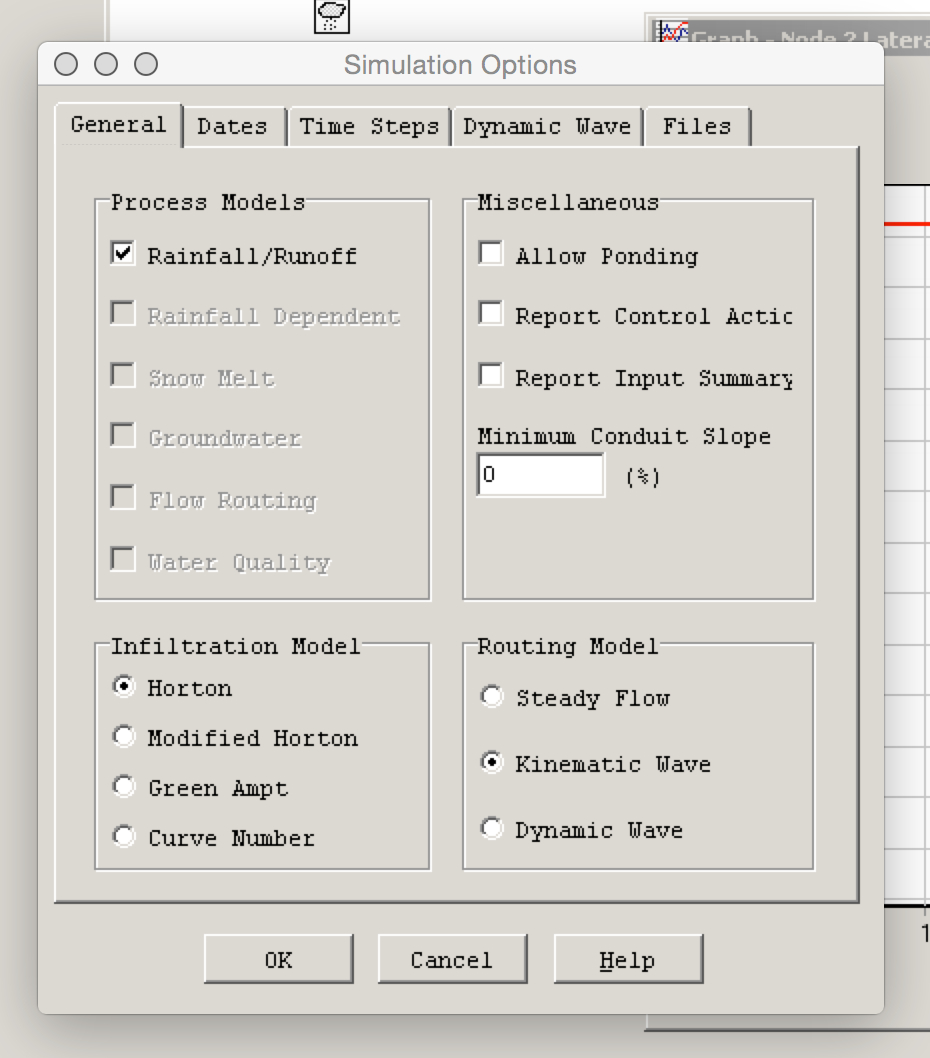
\includegraphics[width=3in]{SWMMHydrologyModels.jpg} 
   \caption{Infiltration (Runoff Generation) Models in SWMM}
   \label{fig:SWMMHydrologyModels}
\end{figure}

The rational runoff model is not a distinct option; probably the intent is that such flows would be added at individual nodes (which is certainly a legitimate option).
However, but adjustment of the infiltration model parameters and use of the percent-impervious value allows one to approximate rational runoff behavior directly.

\section*{\small{Rational in SWMM by Example}}

Consider a $10.9$ acre watershed, with a time of concentration $T_c = 49$ minutes, and a rational runoff coefficient of $0.32$.  
Suppose that the estimated rainfall depth for $45$ minutes is $0.87$ inches.

There is no need for SWMM for just the rational method calculation, but if further hydraulic modeling is needed (perhaps to design a storm sewer or check backwater conditions) then one might have a need to approximate the rational response.

These values in the rational model produce the following results for intensity;
\begin{equation}
i = \frac{0.87\text{ inches}}{49\text{ minutes}} \times 60\text{ minutes per hour} = 1.06 \text{ inches per hour}
\end{equation}

and for peak discharge;

\begin{equation}
Q_p = (0.32) \times 1.06 \text{ inches per hour} \times 10.9 \text{ acres} \approx 3.7 \text{ cubic feet per second}
\end{equation}

For SWMM modeling we need to remember that the peak discharge should occur at around $50$ minutes of constant intensity rainfall of $1.06$ inches per hour.

Now let's build an equivalent model in SWMM and adjust the parameters to approximate the rational equation behavior.

\begin{figure}[h!] %  figure placement: here, top, bottom, or page
   \centering
   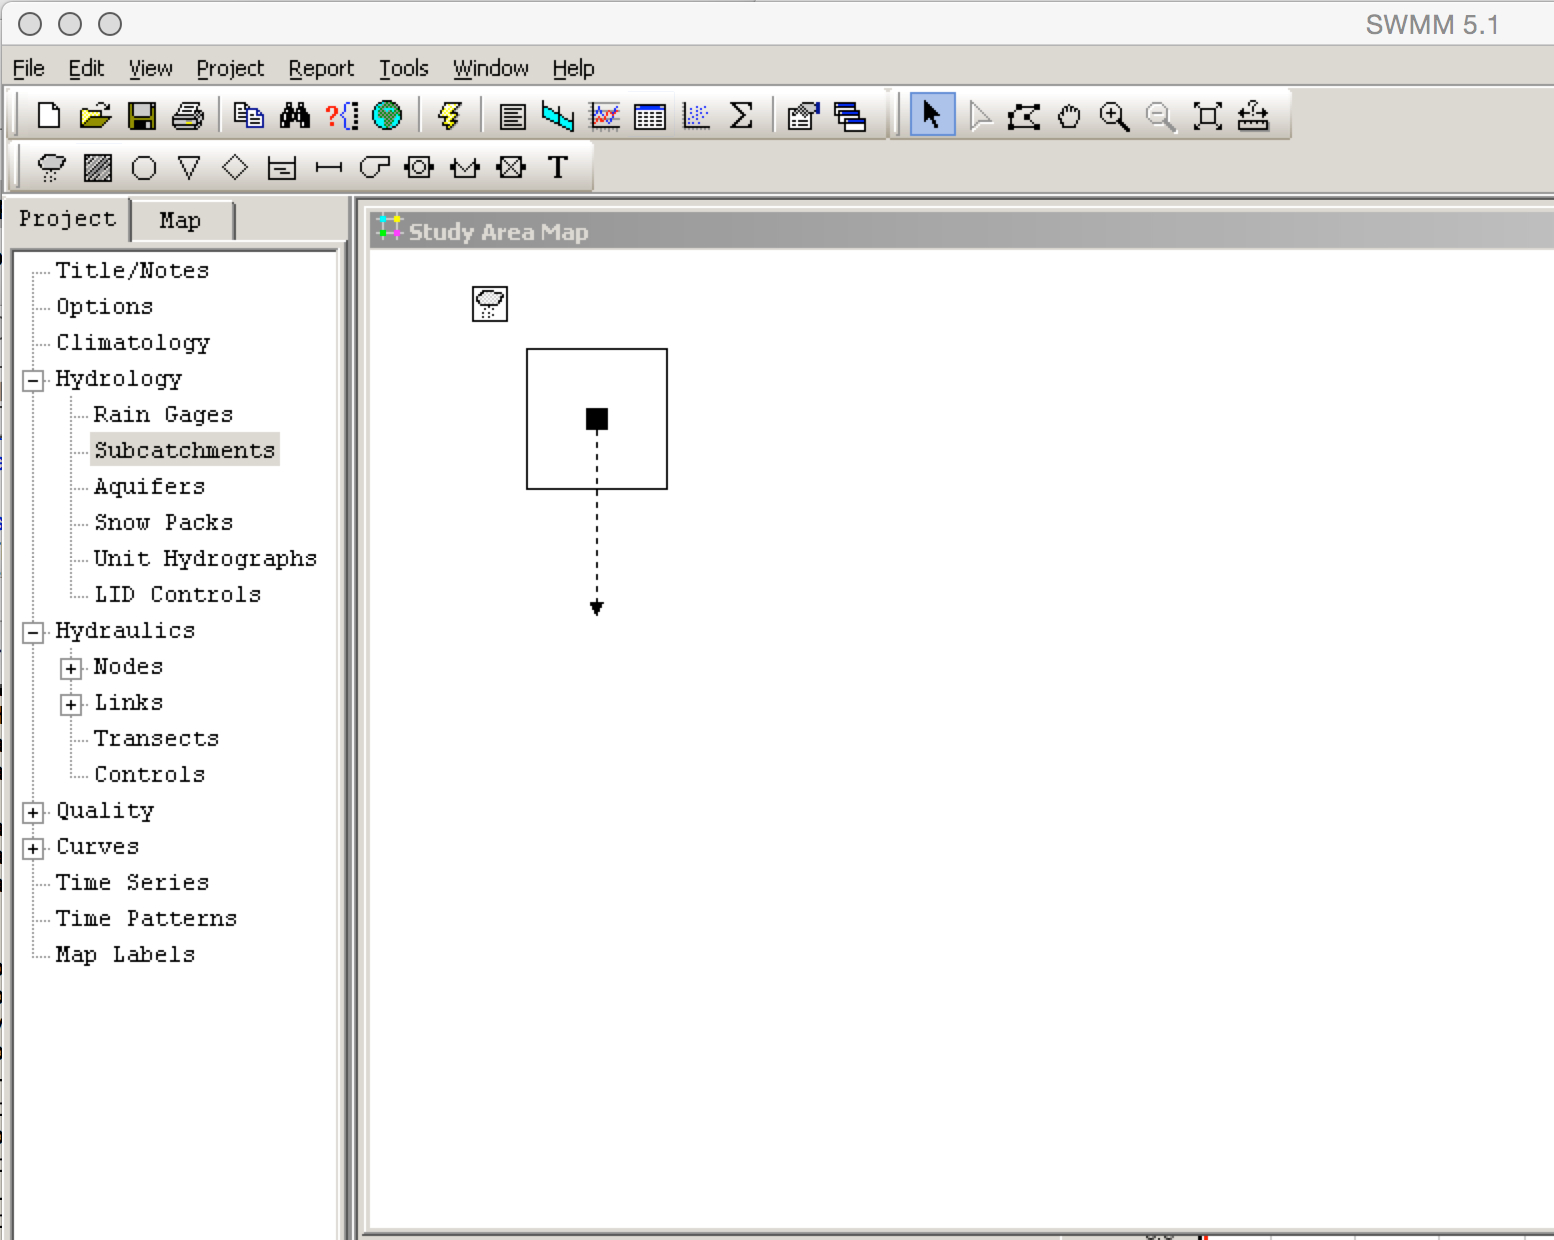
\includegraphics[width=4in]{SWMM-ModelStudyMap.jpg} 
   \caption{Simple Rain gage, Sub-catchment, Outlet SWMM model}
   \label{fig:SWMM-ModelStudyMap}
\end{figure}
Figure \ref{fig:SWMM-ModelStudyMap} is a screen capture of the relatively simple situation described.   
The SWMM model in this example is comprised of three components: the rain gage, the sub-catchment, and the outfall. 
As SWMM models go, this one is pretty minimal.

The rain gage will provide the input for the sub-catchment of $1.06$ inches per hour.
Figure \ref{fig:SWMMRainGage} is a screen capture of the rain gage data entry dialog boxes.

\begin{figure}[h!] %  figure placement: here, top, bottom, or page
   \centering
   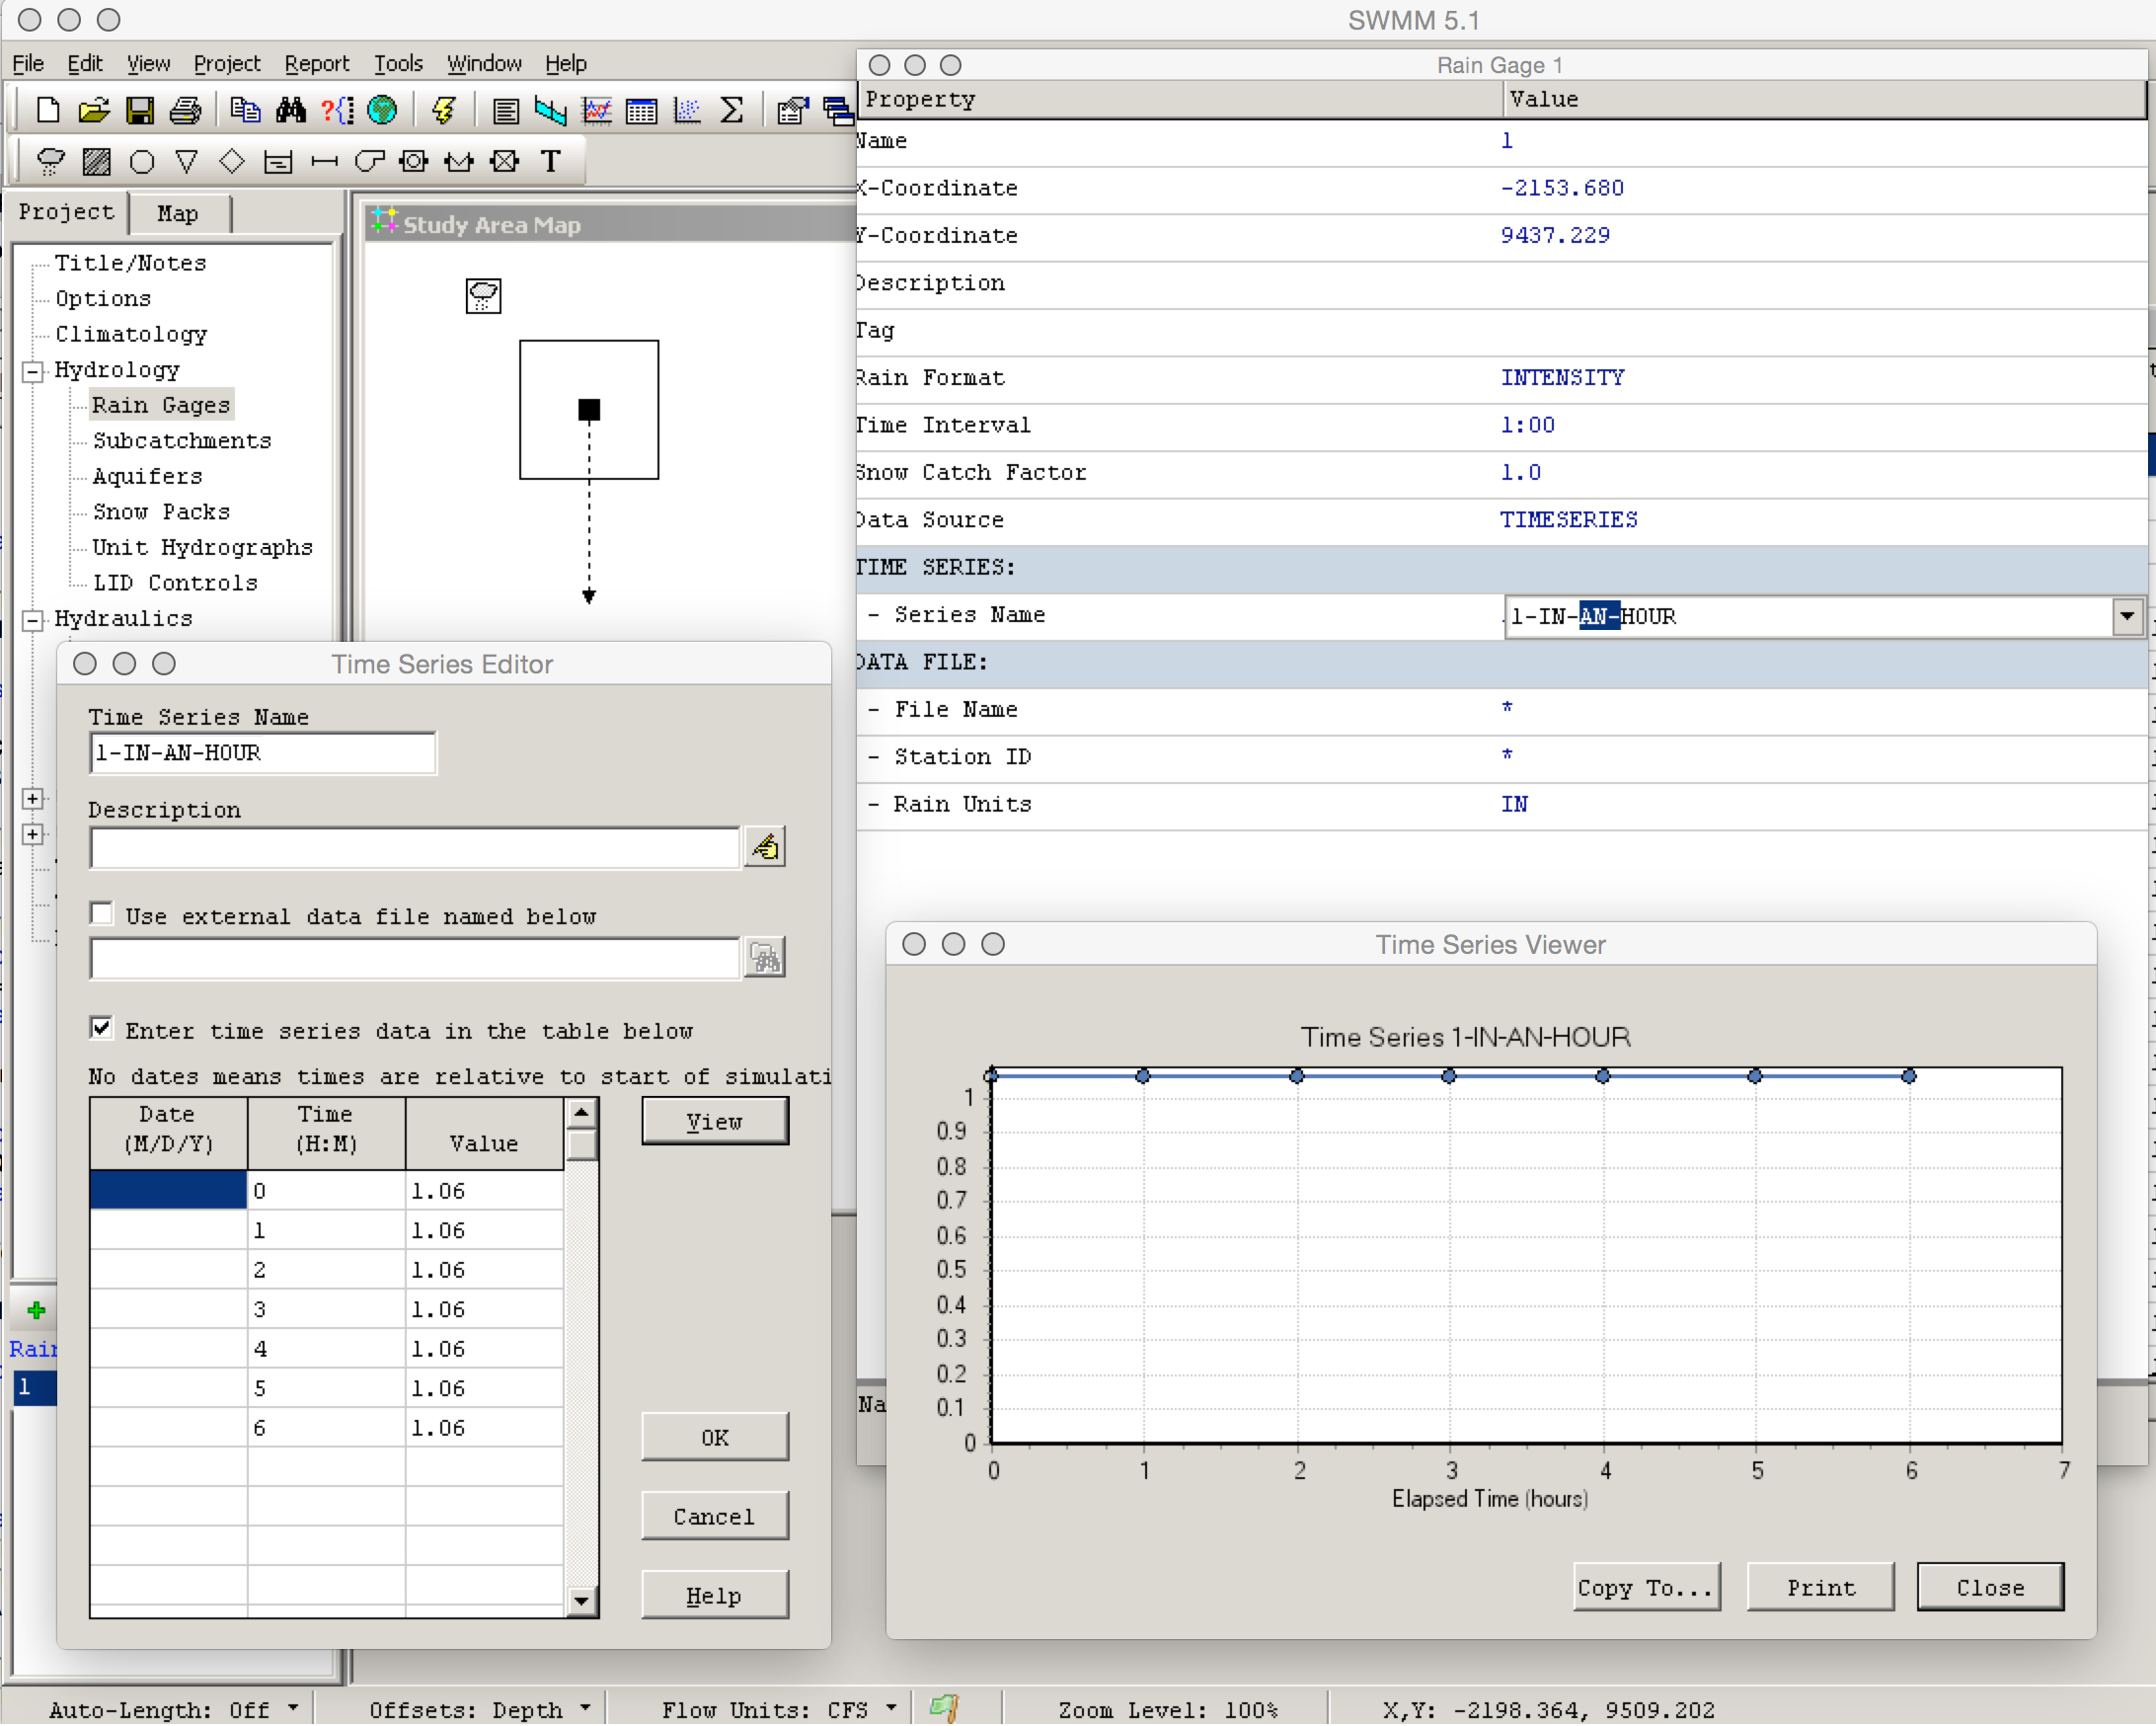
\includegraphics[width=4in]{SWMMRainGage.jpg} 
   \caption{Data entry -- Rain Gage 1 in SWMM}
   \label{fig:SWMMRainGage}
\end{figure}

In the rain gage main dialog, we have selected \texttt{INTENSITY} as the rain format, and a rain gage time increment of $1:00$ hour.  
\footnote{The report time can be a different value; the program works best when the rain gage time step is equal to or larger than the report time step.}
In the time series editor we have entered six hours of the constant rate of $1.06$ inches per hour.   
Six hours should be enough to reach equilibrium, given that we will adjust the inputs so that the peak discharge occurs at $50$ minutes.

Next we create and parameterize the sub-catchment.  This step will take a little trial-and-error but it (the trial-and-error) goes quickly.   
First, make the sub-catchment and set the area ($10.9$ acres).
Then set the \%-Impervious to $100$.   
We also zero a few things.   
Assuming you know the slope, you can put the best value for slope into the dialog box.
Now for the trial-and-error portion.
At $100 \%$ impervious the watershed should produce a peak runoff of
\begin{equation}
Q_{p~100\%}=1.008 \times 1.06\text{ inches per hour} \times 10.9\text{ acres} \approx 11.65\text{ cubic feet per second}
\end{equation}

We use this value to adjust the width in SWMM to make this value occur at $50$ minutes.\footnote{I choose $50$ minutes because it is close to $49$ minutes and one can use $5$ minute reporting times.}
The default width is $500$ feet -- if we know actual slopes and widths, then the only remaining adjustment is the Manning's n value for impervious cover.

Figure \ref{fig:SWMMSubCatchment} is a screen capture of the sub-catchment main dialog box where such adjustments are made. 
On the right side of the figure is the computed runoff in SWMM, the peak discharge is at (00:01:35), which is later in time than the anticipated (00:50:00).
So either the slope needs to be increased (to speed up the outflow), or the Manning's n increased (same reason), or the sub-catchment width increased (to shorten the travel path).

\begin{figure}[h!] %  figure placement: here, top, bottom, or page
   \centering
   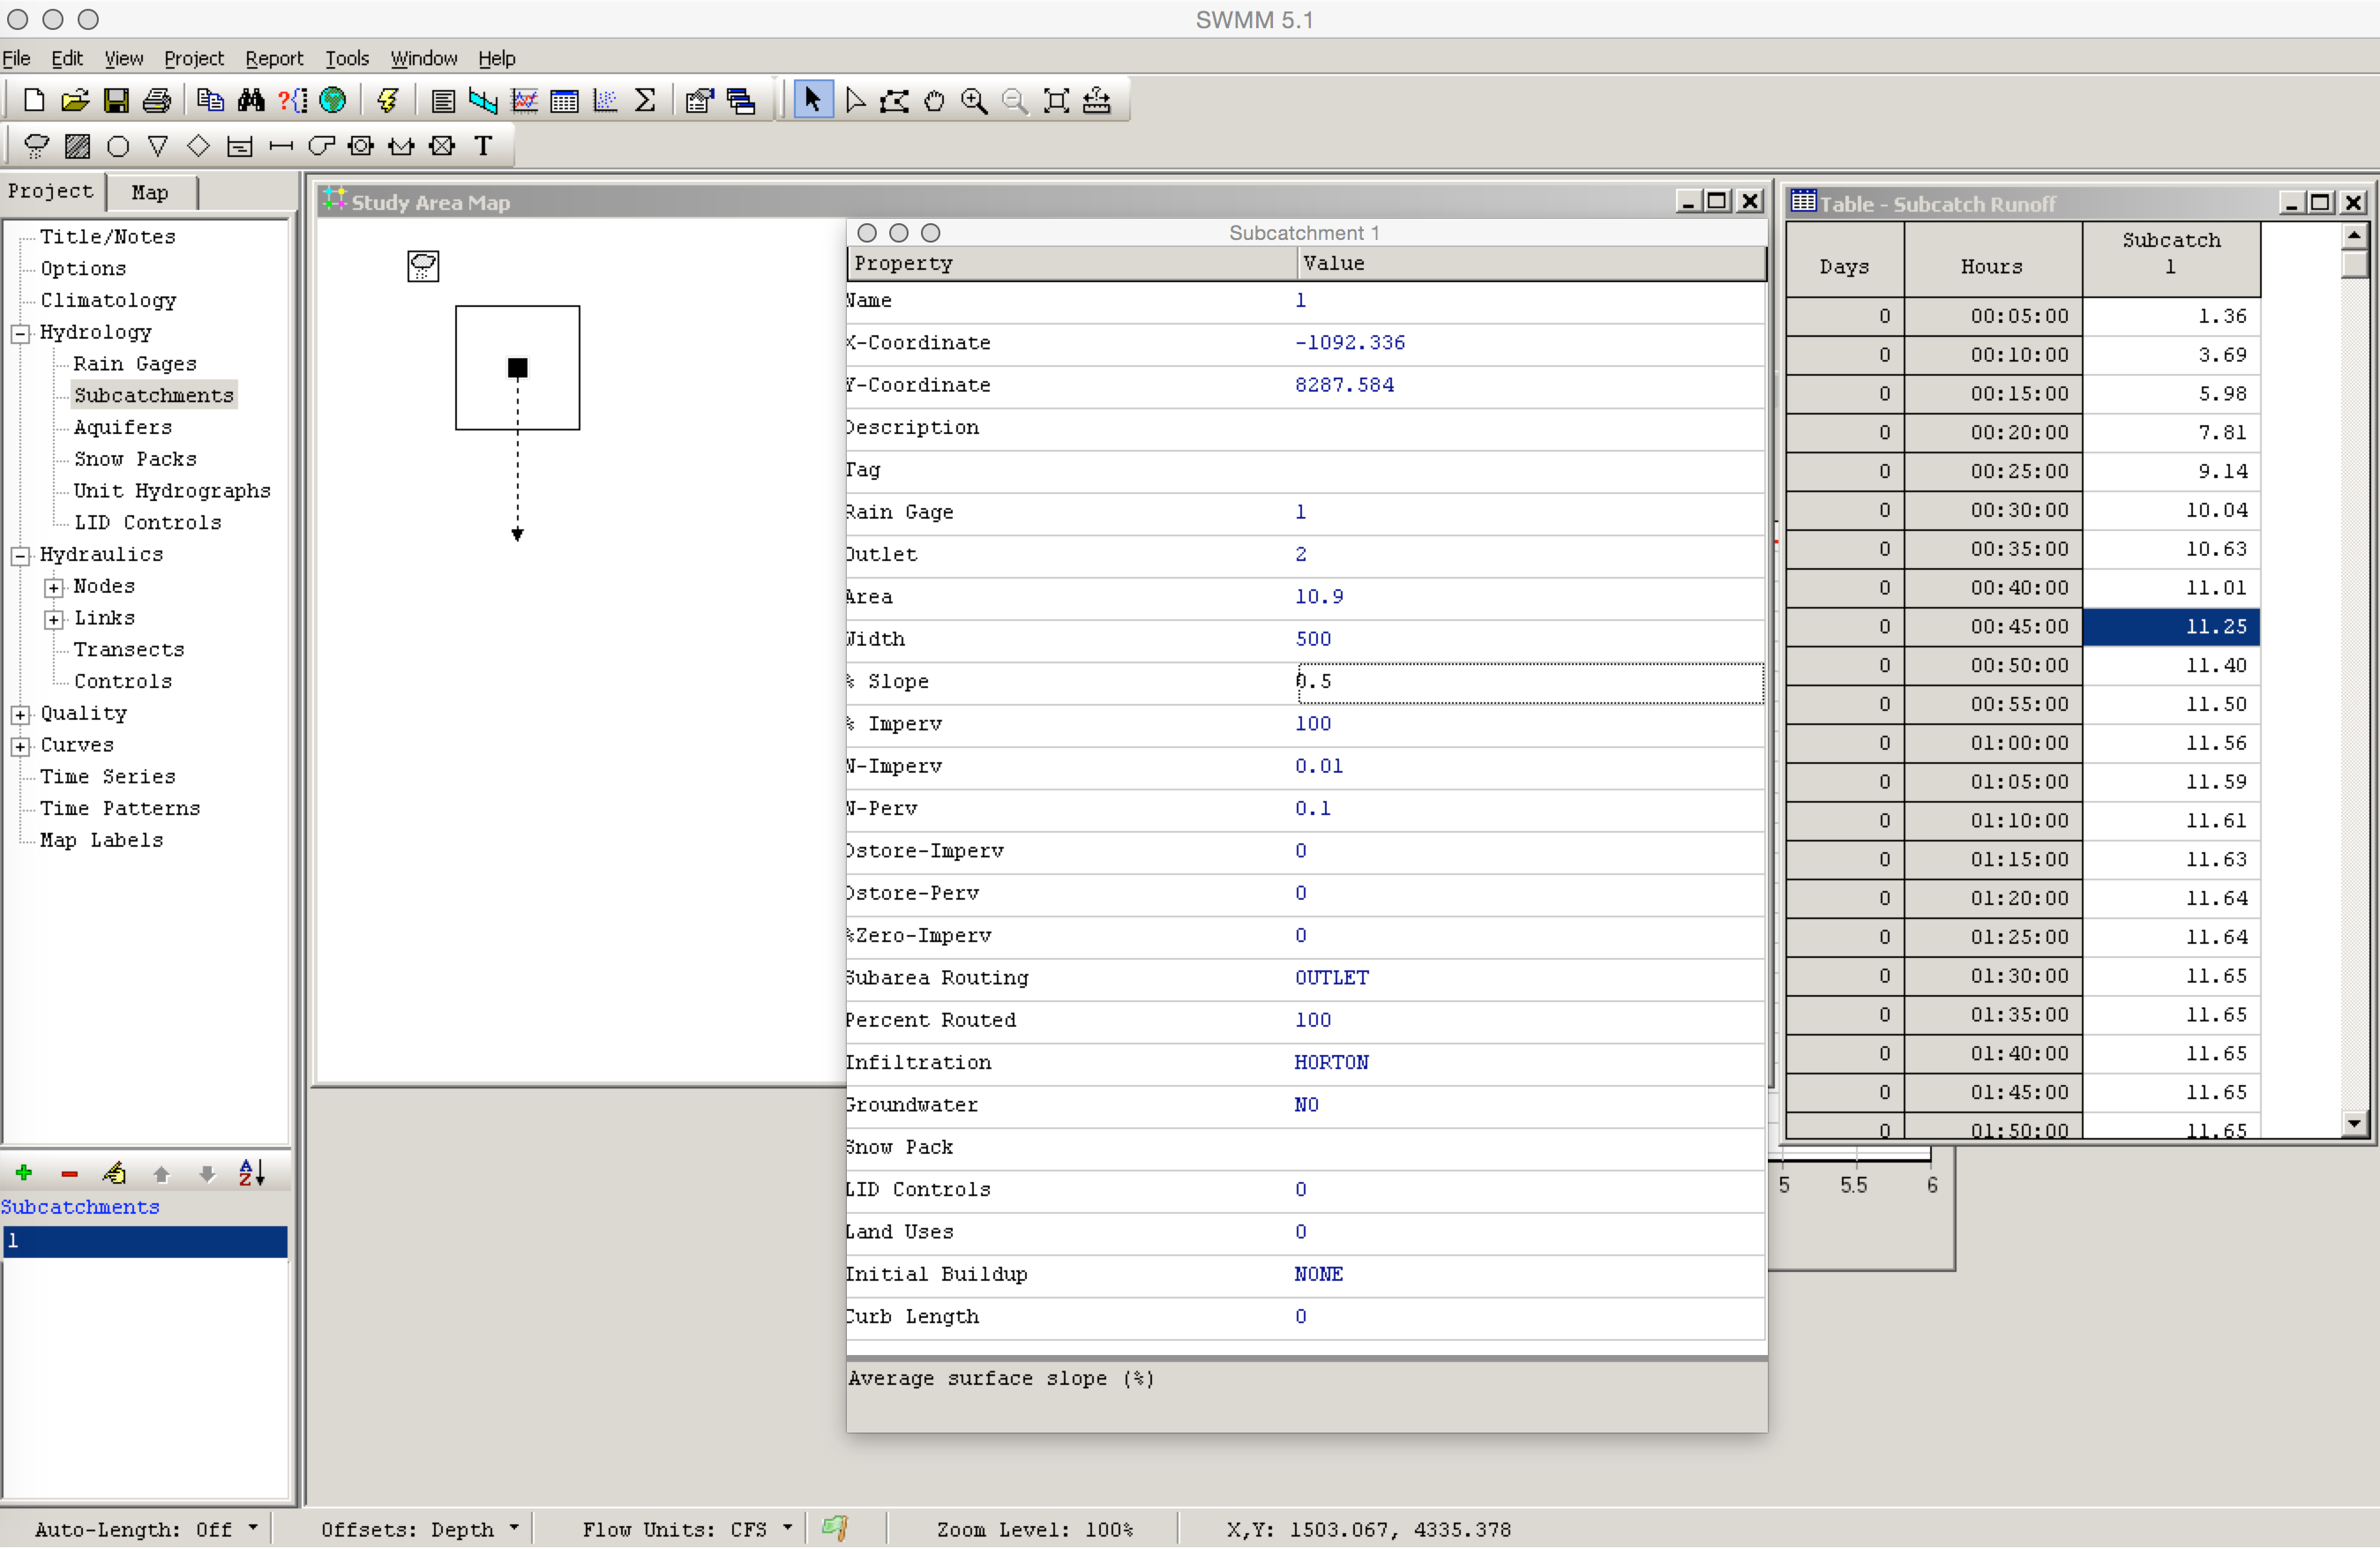
\includegraphics[width=6in]{SWMMSubCatchment.jpg} 
   \caption{Data entry -- Sub-catchment in SWMM}
   \label{fig:SWMMSubCatchment}
\end{figure}

In this example, I am going to increase the width until the peak occurs at (00:50:00).  
Doubling the width changes the time when peak discharge is computed to (01:00:00), which is close.  
A value of $1500$ feet gets the time when the peak arrives to the desired (00:50:00).

Figure \ref{fig:SWMMCalibratedTiming} is a screen capture of the SWMM model now ``adjusted'' so the timing is consistent with the rational method.

\begin{figure}[h!] %  figure placement: here, top, bottom, or page
   \centering
   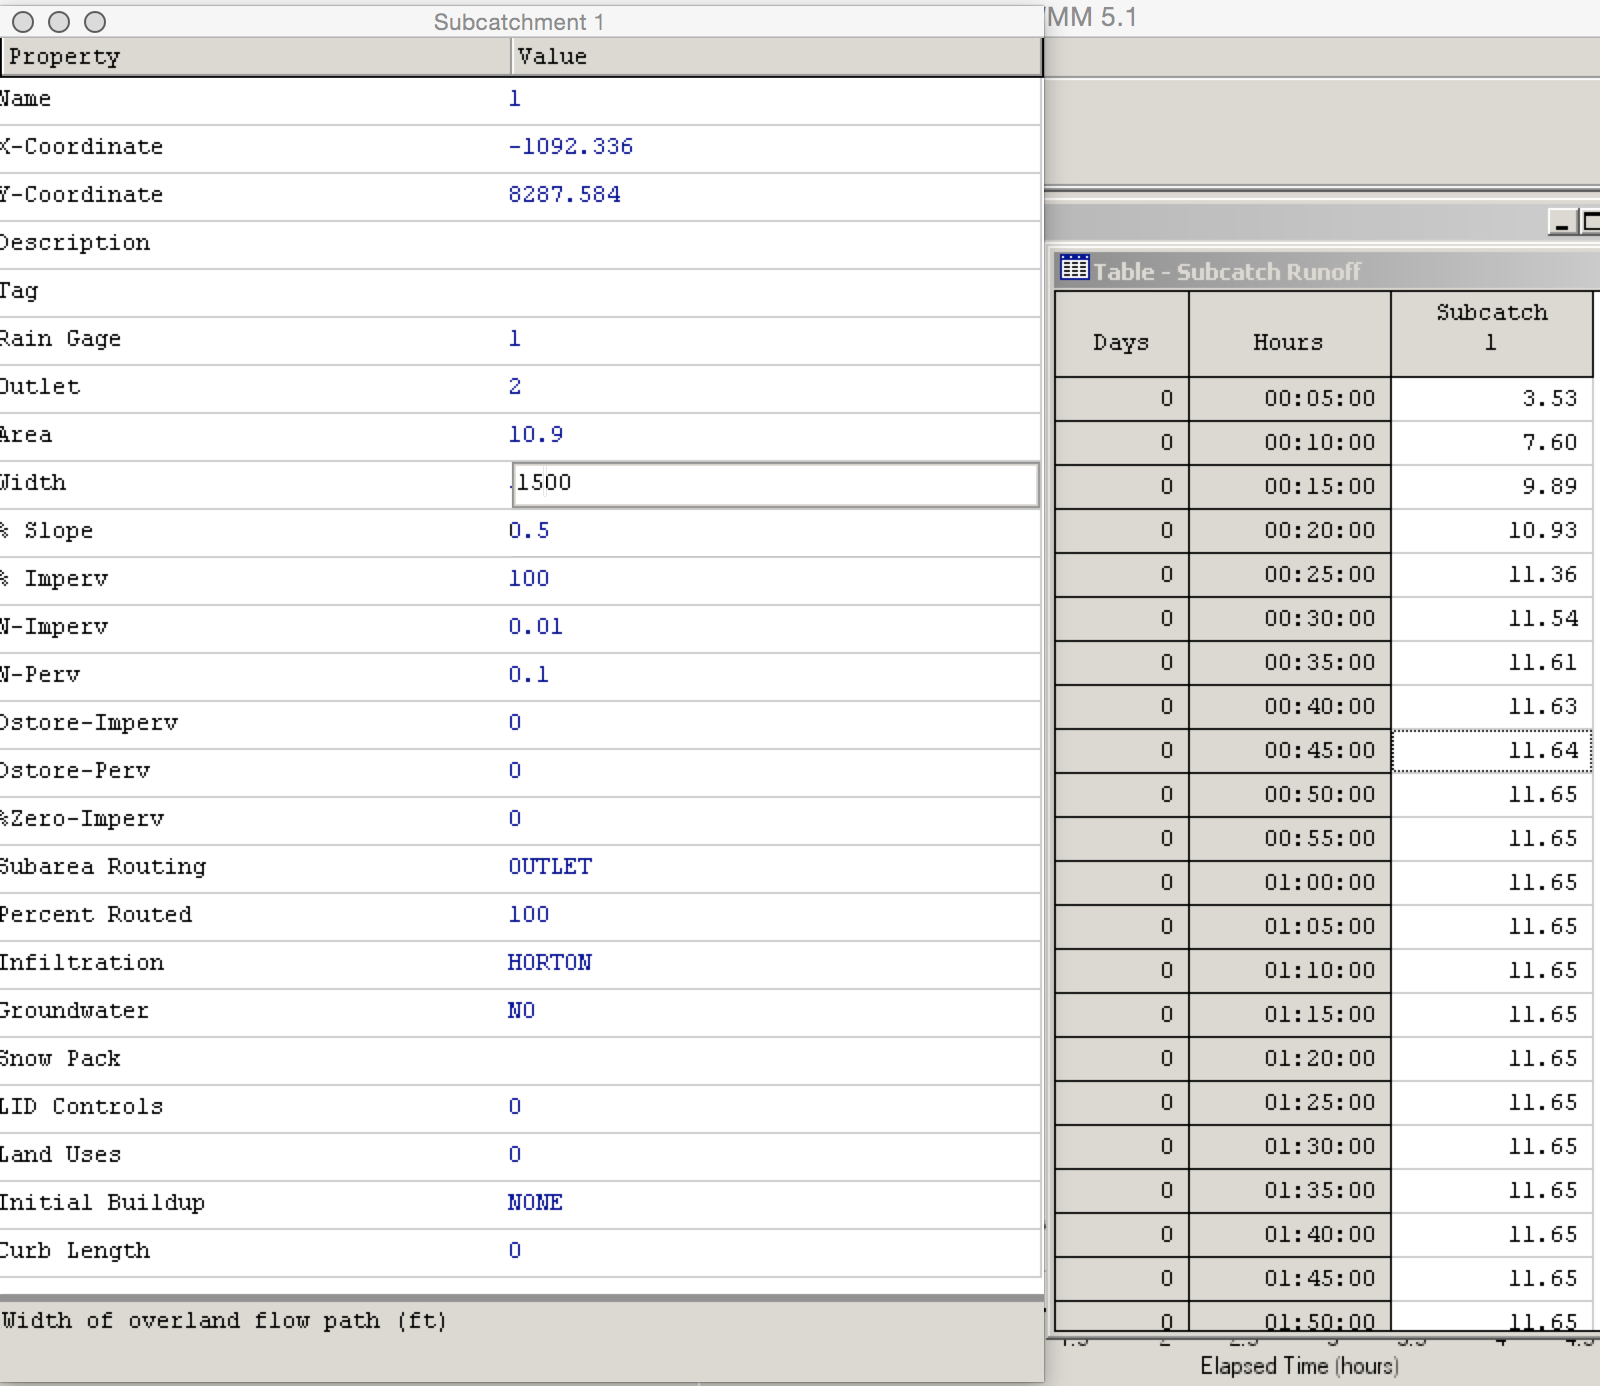
\includegraphics[width=6in]{SWMMCalibratedTiming.jpg} 
   \caption{SWMM Model -- Timing consistent}
   \label{fig:SWMMCalibratedTiming}
\end{figure}

Next we will change the infiltration model parameters so that any rainfall on the pervious portion is completely absorbed (lost) and then the precent impervious value functions as the runoff coefficient.

The key change is to set the infiltration parameters to values that guarantee negligible runoff generation from the pervious portion of a sub-catchment.  
In the case of the Horton model, the initial and asymptotic rates need to be set to large values (larger than the input rainfall rate works nicely).  
Once the changes are made, then we have built a SWMM implementation of the rational method.  

Figure \ref{fig:SWMMRationalWorkingModel} is a screen capture of the example with the changes to reflect the runoff coefficient.  

\begin{figure}[h!] %  figure placement: here, top, bottom, or page
   \centering
   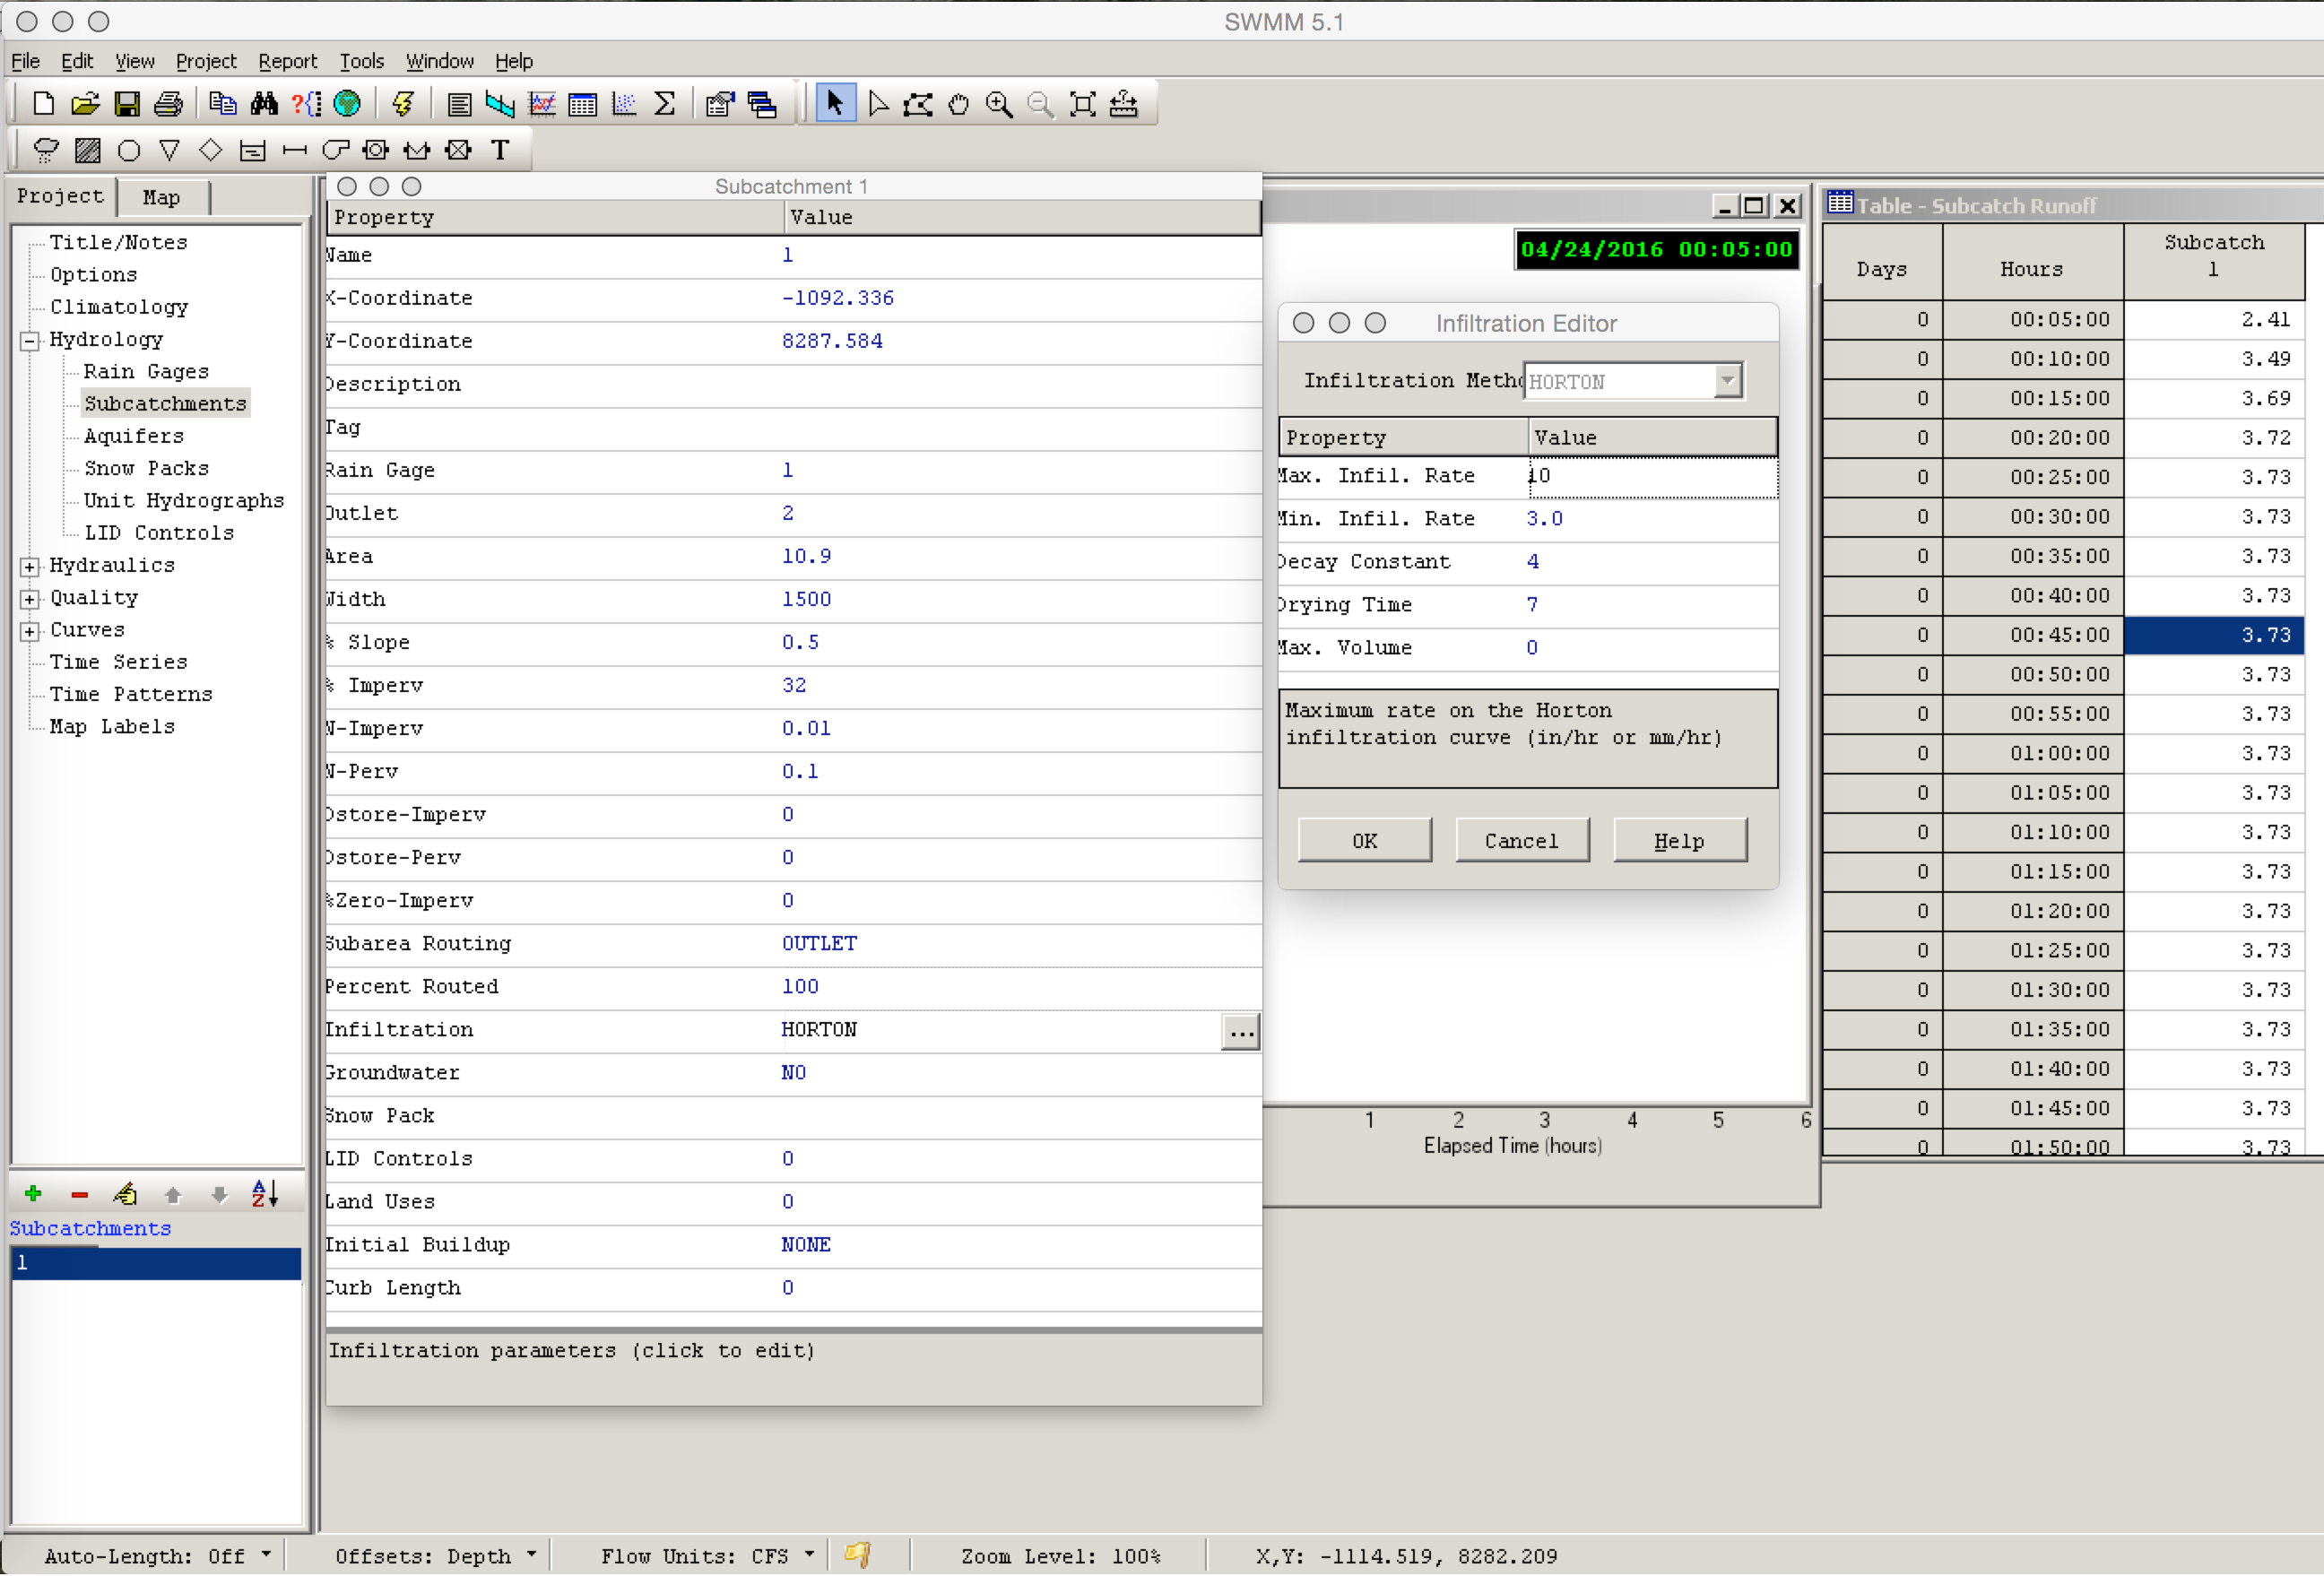
\includegraphics[width=6in]{SWMMRationalWorkingModel.jpg} 
   \caption{Rational runoff approximation using SWMM (Horton) }
   \label{fig:SWMMRationalWorkingModel}
\end{figure}

Notice that the timing is affected -- the timing will never be perfect, but if need to approximate the rational method, we can then use SWMM to test the hydraulics.   
The technique here is useful when one has to match a system that was designed using the rational method and wants the hydrology to be comparable.\footnote{Such a situation arises when using SWMM to forensically test a system that was designed using the rational method -- build the model to replicate the various rational method drainage areas, then apply the historical storm of interest to evaluate the anticipated performance of the system.}
\clearpage

\section*{\small{Addendum}}
The example was presented using Horton's model, but the Green-Ampt models is equally adaptable.  Figure \ref{fig:SWMMRationalGreenAmptModel} is the same example, except the underlying infiltration models were changed.   Notice how the infiltration parameters are selected to ensure complete loss on the pervious parts of the sub-catchment.



\begin{figure}[h!] %  figure placement: here, top, bottom, or page
   \centering
   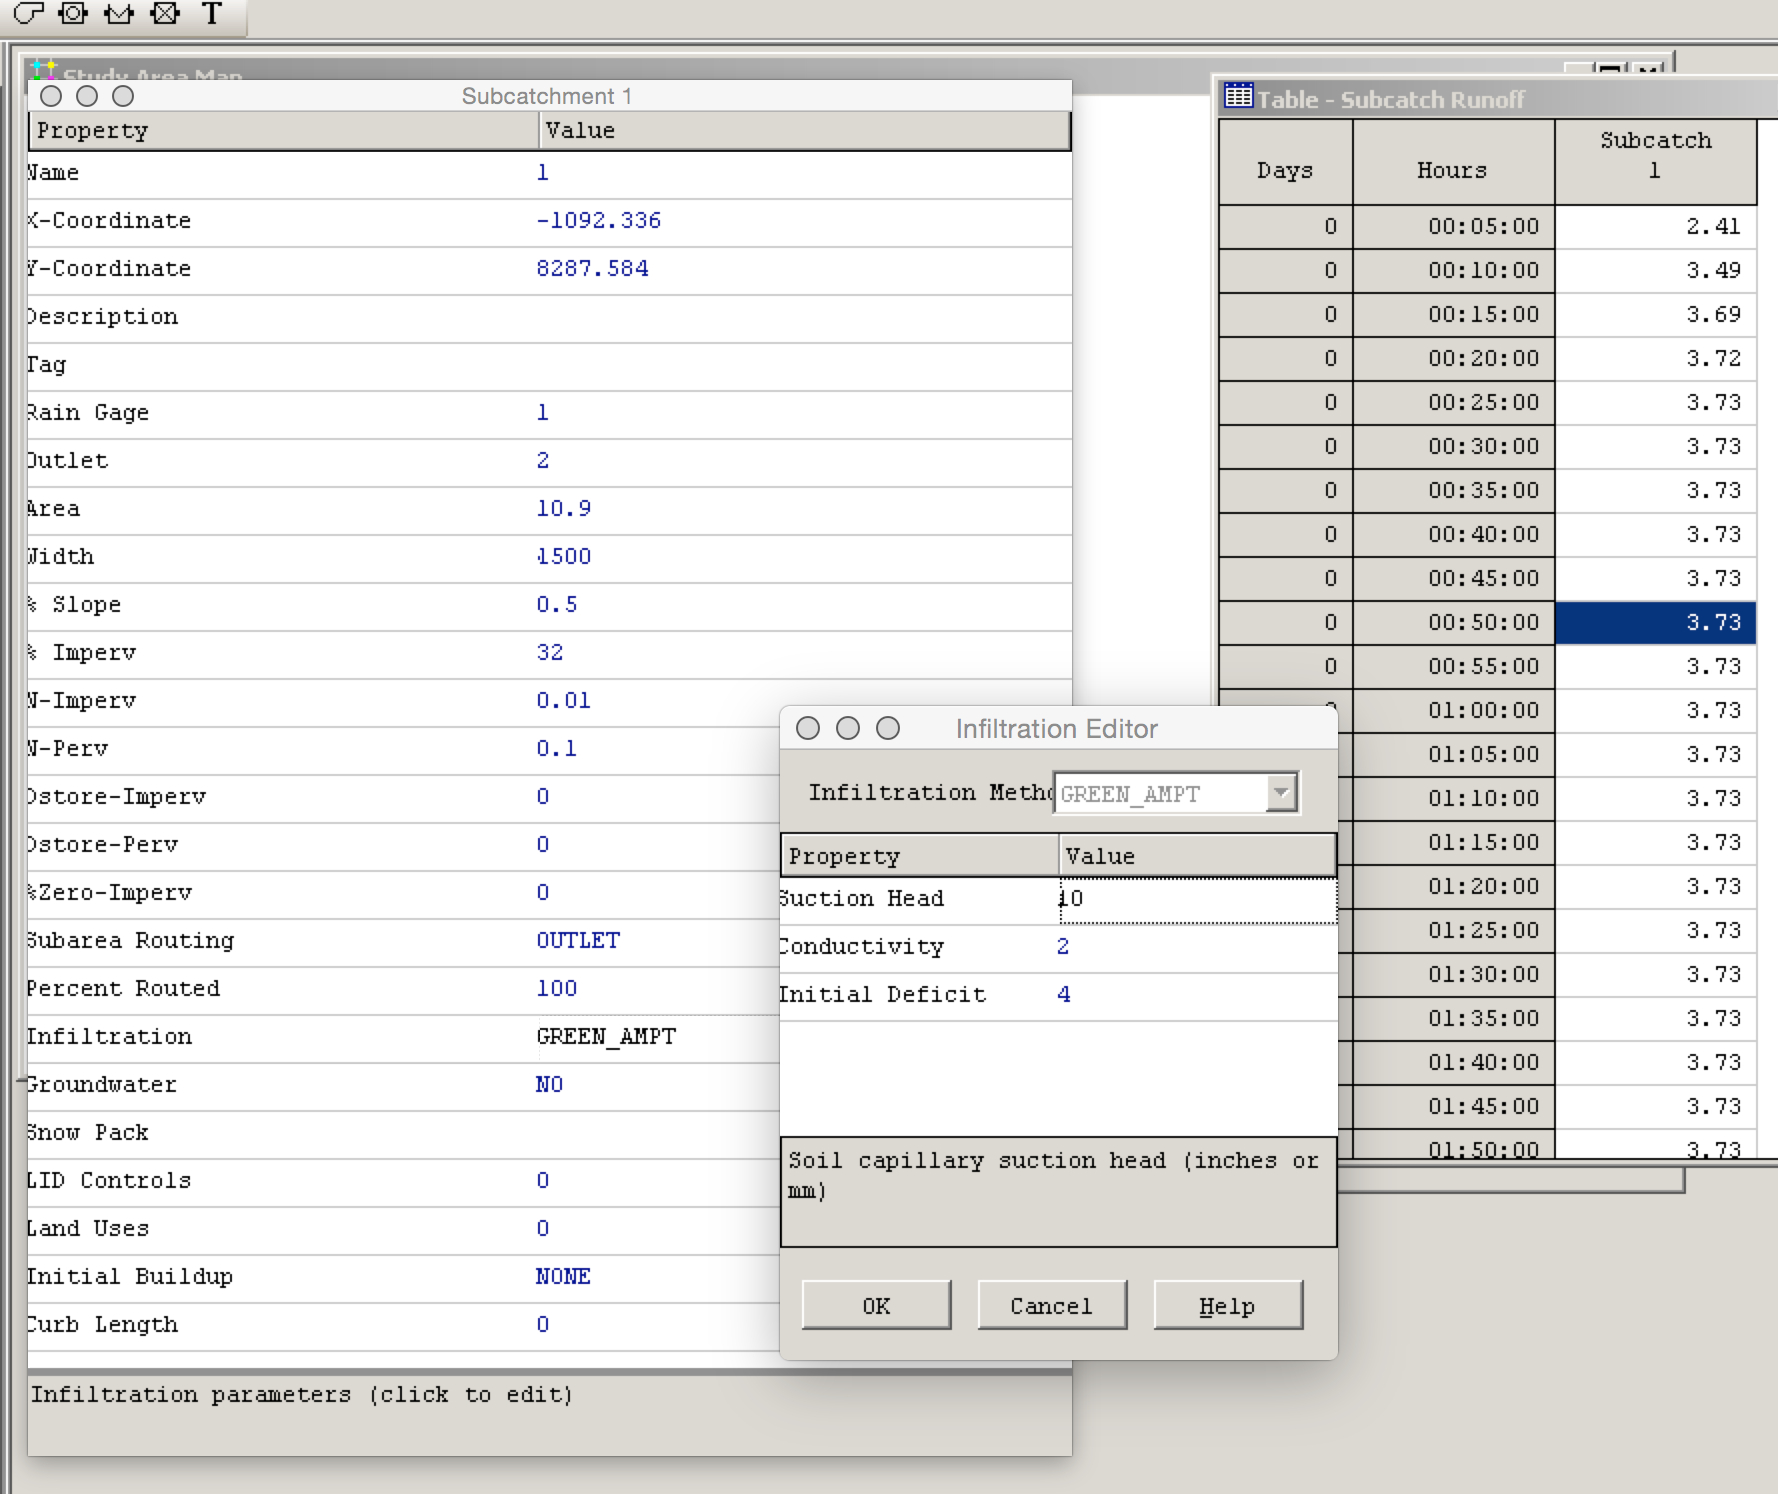
\includegraphics[width=4in]{SWMMRationalGreenAmptModel.jpg} 
   \caption{Rational runoff approximation using SWMM (Green-Ampt) }
   \label{fig:SWMMRationalGreenAmptModel}
\end{figure}

The NRCS Curve Number model is not adaptable into the rational method.  Even a curve number of $0$ in SWMM produces a non-zero runoff value.
%\footnote{This is possibly a flaw in the program's implementation -- although unlikely, or the consequence of how the CN model is implemented in a time-varying environment.  Either way, the CN approach is difficult to match to the rational runoff model.}




\end{document}  